\section{Register description}
\regover{
{\hyperref[ir-irtx-config]{irtx\_config}}&
\\
\hline
{\hyperref[ir-irtx-int-sts]{irtx\_int\_sts}}&
\\
\hline
{\hyperref[ir-irtx-pulse-width]{irtx\_pulse\_width}}&
\\
\hline
{\hyperref[ir-irtx-pw-0]{irtx\_pw\_0}}&
\\
\hline
{\hyperref[ir-irtx-pw-1]{irtx\_pw\_1}}&
\\
\hline
{\hyperref[ir-irrx-config]{irrx\_config}}&
\\
\hline
{\hyperref[ir-irrx-int-sts]{irrx\_int\_sts}}&
\\
\hline
{\hyperref[ir-irrx-pw-config]{irrx\_pw\_config}}&
\\
\hline
{\hyperref[ir-irrx-data-count]{irrx\_data\_count}}&
\\
\hline
{\hyperref[ir-irrx-data-word0]{irrx\_data\_word0}}&
\\
\hline
{\hyperref[ir-irrx-data-word1]{irrx\_data\_word1}}&
\\
\hline
{\hyperref[ir-irtx-fifo-config-0]{irtx\_fifo\_config\_0}}&
\\
\hline
{\hyperref[ir-irtx-fifo-config-1]{irtx\_fifo\_config\_1}}&
\\
\hline
{\hyperref[ir-ir-fifo-wdata]{ir\_fifo\_wdata}}&
\\
\hline
{\hyperref[ir-ir-fifo-rdata]{ir\_fifo\_rdata}}&
\\
\hline
}

\subsection{irtx\_config}
\label{ir-irtx-config}
Address:0x2000a600
 \begin{figure}[H]
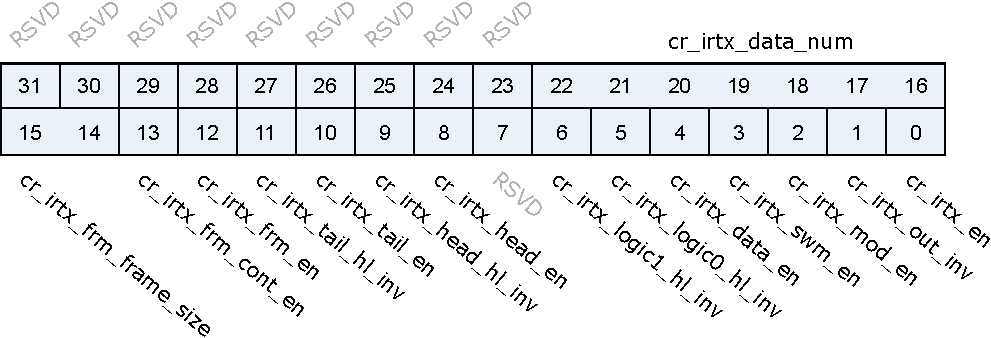
\includegraphics{ir_irtx_config.pdf}
\end{figure}

\regdes{31:23&RSVD& & & \\\hline
22:16&cr\_irtx\_data\_num&r/w&7'd31&Bit count of Data phase (unit: bit / PW for normal / SWM) \par (Don't-care if cr\_irtx\_frm\_en is enabled)
\\\hline
15:14&cr\_irtx\_frm\_frame\_size&r/w&2'd0&IRTX freerun mode frame size (also the valid width for each FIFO entry) \par 2'd0: 8-bit \par 2'd1: 16-bit \par 2'd2: 24-bit \par 2'd3: 32-bit
\\\hline
13&cr\_irtx\_frm\_cont\_en&r/w&1'b0&Enable signal of IRTX freerun continuous mode \par 0: Disabled, each data frame is separated by an idle time (tail\_ph0\_w+1 + tail\_ph1\_w+1)*pw\_unit \par 1: Enabled, data continuously sent without interval (if FIFO data is valid)
\\\hline
12&cr\_irtx\_frm\_en&r/w&1'b0&Enable signal of IRTX freerun mode (Don't care if SWM is enabled) \par Note: HEAD/TAIL is disabled in freerun mode
\\\hline
11&cr\_irtx\_tail\_hl\_inv&r/w&1'b0&Tail pulse H/L inverse signal (Don't care if SWM or FRM is enabled) \par 0: Phase 0 is High (Active), phase 1 is Low (Idle) (H -> L) \par 1: Phase 0 is Low (Idle), phase 1 is High (Active) (L -> H)
\\\hline
10&cr\_irtx\_tail\_en&r/w&1'b1&Enable signal of tail pulse (Don't care if SWM or FRM is enabled)\\\hline
9&cr\_irtx\_head\_hl\_inv&r/w&1'b0&Tail pulse H/L inverse signal (Don't care if SWM or FRM is enabled) \par 0: Phase 0 is High (Active), phase 1 is Low (Idle) (H -> L) \par 1: Phase 0 is Low (Idle), phase 1 is High (Active) (L -> H)
\\\hline
8&cr\_irtx\_head\_en&r/w&1'b1&Enable signal of head pulse (Don't care if SWM or FRM is enabled)\\\hline
7&RSVD& & & \\\hline
6&cr\_irtx\_logic1\_hl\_inv&r/w&1'b0&Logic 1 H/L inverse signal (Don't care if SWM is enabled) \par 0: Phase 0 is High (Active), phase 1 is Low (Idle) (H -> L) \par 1: Phase 0 is Low (Idle), phase 1 is High (Active) (L -> H)
\\\hline
5&cr\_irtx\_logic0\_hl\_inv&r/w&1'b0&Logic 0 H/L inverse signal (Don't care if SWM is enabled) \par 0: Phase 0 is High (Active), phase 1 is Low (Idle) (H -> L) \par 1: Phase 0 is Low (Idle), phase 1 is High (Active) (L -> H)
\\\hline
4&cr\_irtx\_data\_en&r/w&1'b1&Enable signal of data phase (Don't care if SWM or FRM is enabled)\\\hline
3&cr\_irtx\_swm\_en&r/w&1'b0&Enable signal of IRTX Software Mode (SWM)\\\hline
2&cr\_irtx\_mod\_en&r/w&1'b0&Enable signal of output modulation\\\hline
1&cr\_irtx\_out\_inv&r/w&1'b0&Output inverse signal \par 1'b0: Output stays at Low during idle state \par 1'b1: Output stays at High during idle state
\\\hline
0&cr\_irtx\_en&r/w&1'b0&Enable signal of IRTX function \par Asserting this bit will trigger the transaction, and should be de-asserted after finish
\\\hline

}
\subsection{irtx\_int\_sts}
\label{ir-irtx-int-sts}
Address:0x2000a604
 \begin{figure}[H]
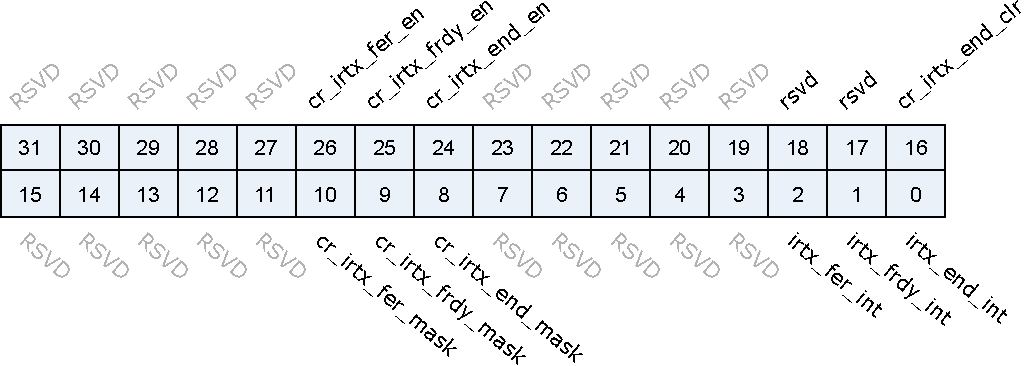
\includegraphics{ir_irtx_int_sts.pdf}
\end{figure}

\regdes{31:27&RSVD& & & \\\hline
26&cr\_irtx\_fer\_en&r/w&1'b1&Interrupt enable of irtx\_fer\_int\\\hline
25&cr\_irtx\_frdy\_en&r/w&1'b1&Interrupt enable of irtx\_frdy\_int\\\hline
24&cr\_irtx\_end\_en&r/w&1'b1&Interrupt enable of irtx\_end\_int\\\hline
23:19&RSVD& & & \\\hline
18&rsvd&rsvd&1'b0&\\\hline
17&rsvd&rsvd&1'b0&\\\hline
16&cr\_irtx\_end\_clr&w1c&1'b0&Interrupt clear of irtx\_end\_int\\\hline
15:11&RSVD& & & \\\hline
10&cr\_irtx\_fer\_mask&r/w&1'b1&Interrupt mask of irtx\_fer\_int\\\hline
9&cr\_irtx\_frdy\_mask&r/w&1'b1&Interrupt mask of irtx\_frdy\_int\\\hline
8&cr\_irtx\_end\_mask&r/w&1'b1&Interrupt mask of irtx\_end\_int\\\hline
7:3&RSVD& & & \\\hline
2&irtx\_fer\_int&r&1'b0&IRTX FIFO error interrupt, auto-cleared when FIFO overflow/underflow error flag is cleared\\\hline
1&irtx\_frdy\_int&r&1'b1&IRTX FIFO ready (tx\_fifo\_cnt > tx\_fifo\_th) interrupt, auto-cleared when data is pushed\\\hline
0&irtx\_end\_int&r&1'b0&IRTX transfer end interrupt\\\hline

}
\subsection{irtx\_pulse\_width}
\label{ir-irtx-pulse-width}
Address:0x2000a610
 \begin{figure}[H]
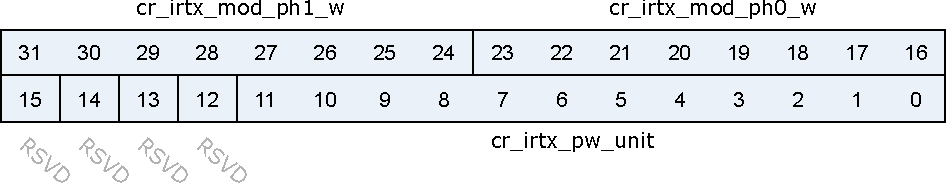
\includegraphics{ir_irtx_pulse_width.pdf}
\end{figure}

\regdes{31:24&cr\_irtx\_mod\_ph1\_w&r/w&8'd34&Modulation phase 1 width\\\hline
23:16&cr\_irtx\_mod\_ph0\_w&r/w&8'd17&Modulation phase 0 width\\\hline
15:12&RSVD& & & \\\hline
11:0&cr\_irtx\_pw\_unit&r/w&12'd1124&Pulse width unit\\\hline

}
\subsection{irtx\_pw\_0}
\label{ir-irtx-pw-0}
Address:0x2000a614
 \begin{figure}[H]
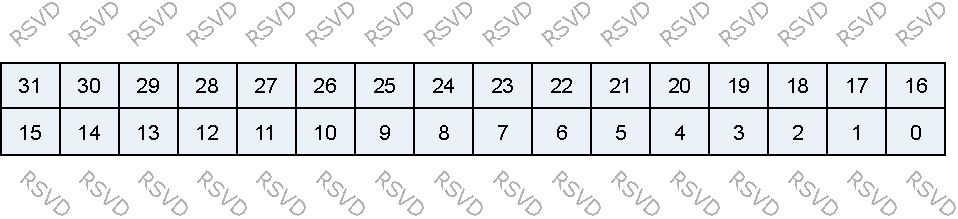
\includegraphics{ir_irtx_pw_0.pdf}
\end{figure}

\regdes{31:24&cr\_irtx\_logic1\_ph1\_w&r/w&8'd2&Pulse width of logic1 phase 1 (Don't care if SWM is enabled)\\\hline
23:16&cr\_irtx\_logic1\_ph0\_w&r/w&8'd0&Pulse width of logic1 phase 0 (Don't care if SWM is enabled)\\\hline
15:8&cr\_irtx\_logic0\_ph1\_w&r/w&8'd0&Pulse width of logic0 phase 1 (Don't care if SWM is enabled)\\\hline
7:0&cr\_irtx\_logic0\_ph0\_w&r/w&8'd0&Pulse width of logic0 phase 0 (Don't care if SWM is enabled)\\\hline

}
\subsection{irtx\_pw\_1}
\label{ir-irtx-pw-1}
Address:0x2000a618
 \begin{figure}[H]
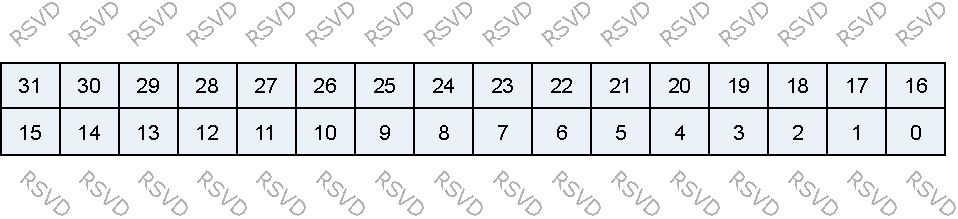
\includegraphics{ir_irtx_pw_1.pdf}
\end{figure}

\regdes{31:24&cr\_irtx\_tail\_ph1\_w&r/w&8'd0&Pulse width of tail pulse phase 1 (Don't care if SWM is enabled)\\\hline
23:16&cr\_irtx\_tail\_ph0\_w&r/w&8'd0&Pulse width of tail pulse phase 0 (Don't care if SWM is enabled)\\\hline
15:8&cr\_irtx\_head\_ph1\_w&r/w&8'd7&Pulse width of head pulse phase 1 (Don't care if SWM is enabled)\\\hline
7:0&cr\_irtx\_head\_ph0\_w&r/w&8'd15&Pulse width of head pulse phase 0 (Don't care if SWM is enabled)\\\hline

}
\subsection{irrx\_config}
\label{ir-irrx-config}
Address:0x2000a640
 \begin{figure}[H]
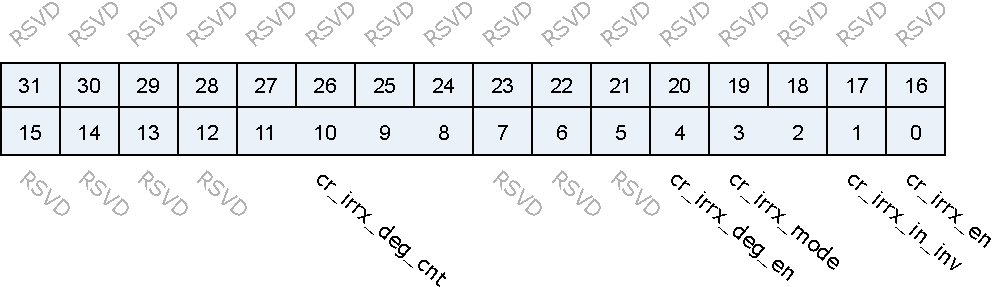
\includegraphics{ir_irrx_config.pdf}
\end{figure}

\regdes{31:12&RSVD& & & \\\hline
11:8&cr\_irrx\_deg\_cnt&r/w&4'd0&De-glitch function cycle count\\\hline
7:5&RSVD& & & \\\hline
4&cr\_irrx\_deg\_en&r/w&1'b0&Enable signal of IRRX input de-glitch function\\\hline
3:2&cr\_irrx\_mode&r/w&2'd0&IRRX mode \par 0: NEC \par 1: RC5 \par 2: SW pulse-width detection mode (SWM) \par 3: Reserved
\\\hline
1&cr\_irrx\_in\_inv&r/w&1'b1&Input inverse signal\\\hline
0&cr\_irrx\_en&r/w&1'b0&Enable signal of IRRX function \par Asserting this bit will trigger the transaction, and should be de-asserted after finish
\\\hline

}
\subsection{irrx\_int\_sts}
\label{ir-irrx-int-sts}
Address:0x2000a644
 \begin{figure}[H]
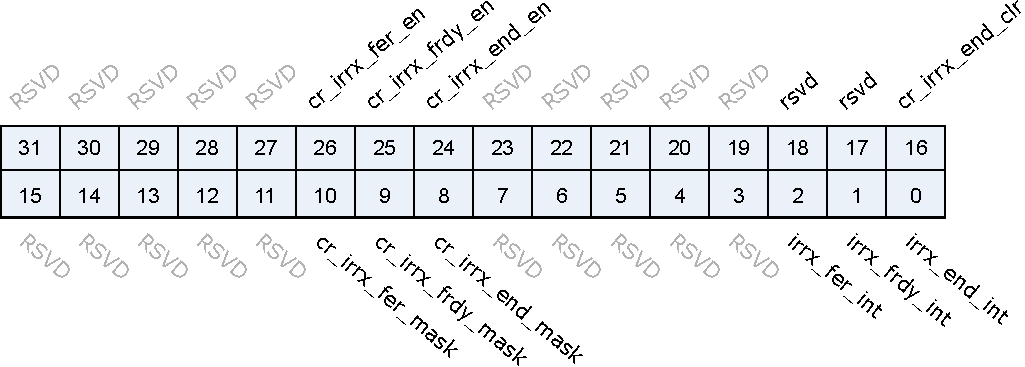
\includegraphics{ir_irrx_int_sts.pdf}
\end{figure}

\regdes{31:27&RSVD& & & \\\hline
26&cr\_irrx\_fer\_en&r/w&1'b1&Interrupt enable of irrx\_fer\_int\\\hline
25&cr\_irrx\_frdy\_en&r/w&1'b1&Interrupt enable of irrx\_frdy\_int\\\hline
24&cr\_irrx\_end\_en&r/w&1'b1&Interrupt enable of irrx\_end\_int\\\hline
23:19&RSVD& & & \\\hline
18&rsvd&rsvd&1'b0&\\\hline
17&rsvd&rsvd&1'b0&\\\hline
16&cr\_irrx\_end\_clr&w1c&1'b0&Interrupt clear of irrx\_end\_int\\\hline
15:11&RSVD& & & \\\hline
10&cr\_irrx\_fer\_mask&r/w&1'b1&Interrupt mask of irrx\_fer\_int\\\hline
9&cr\_irrx\_frdy\_mask&r/w&1'b1&Interrupt mask of irrx\_frdy\_int\\\hline
8&cr\_irrx\_end\_mask&r/w&1'b1&Interrupt mask of irrx\_end\_int\\\hline
7:3&RSVD& & & \\\hline
2&irrx\_fer\_int&r&1'b0&IRRX FIFO error interrupt, auto-cleared when FIFO overflow/underflow error flag is cleared\\\hline
1&irrx\_frdy\_int&r&1'b0&IRRX FIFO ready (rx\_fifo\_cnt > rx\_fifo\_th) interrupt, auto-cleared when data is popped\\\hline
0&irrx\_end\_int&r&1'b0&IRRX transfer end interrupt\\\hline

}
\subsection{irrx\_pw\_config}
\label{ir-irrx-pw-config}
Address:0x2000a648
 \begin{figure}[H]
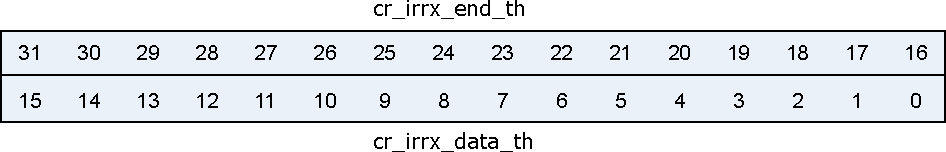
\includegraphics{ir_irrx_pw_config.pdf}
\end{figure}

\regdes{31:16&cr\_irrx\_end\_th&r/w&16'd8999&Pulse width threshold to trigger END condition\\\hline
15:0&cr\_irrx\_data\_th&r/w&16'd3399&Pulse width threshold for Logic0/1 detection (Don't care if SWM is enabled)\\\hline

}
\subsection{irrx\_data\_count}
\label{ir-irrx-data-count}
Address:0x2000a650
 \begin{figure}[H]
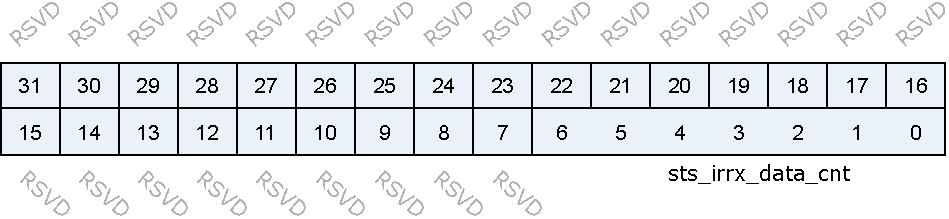
\includegraphics{ir_irrx_data_count.pdf}
\end{figure}

\regdes{31:7&RSVD& & & \\\hline
6:0&sts\_irrx\_data\_cnt&r&7'd0&RX data bit count (pulse-width count for SWM)\\\hline

}
\subsection{irrx\_data\_word0}
\label{ir-irrx-data-word0}
Address:0x2000a654
 \begin{figure}[H]
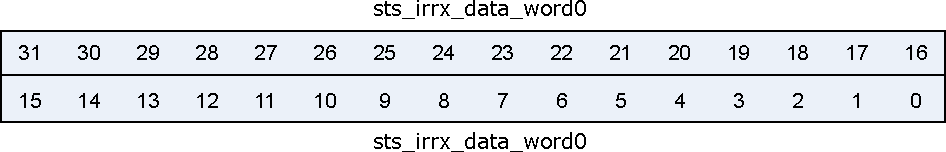
\includegraphics{ir_irrx_data_word0.pdf}
\end{figure}

\regdes{31:0&sts\_irrx\_data\_word0&r&32'h0&RX data word 0\\\hline

}
\subsection{irrx\_data\_word1}
\label{ir-irrx-data-word1}
Address:0x2000a658
 \begin{figure}[H]
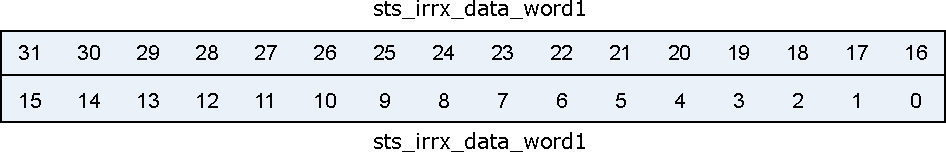
\includegraphics{ir_irrx_data_word1.pdf}
\end{figure}

\regdes{31:0&sts\_irrx\_data\_word1&r&32'h0&RX data word 1\\\hline

}
\subsection{irtx\_fifo\_config\_0}
\label{ir-irtx-fifo-config-0}
Address:0x2000a680
 \begin{figure}[H]
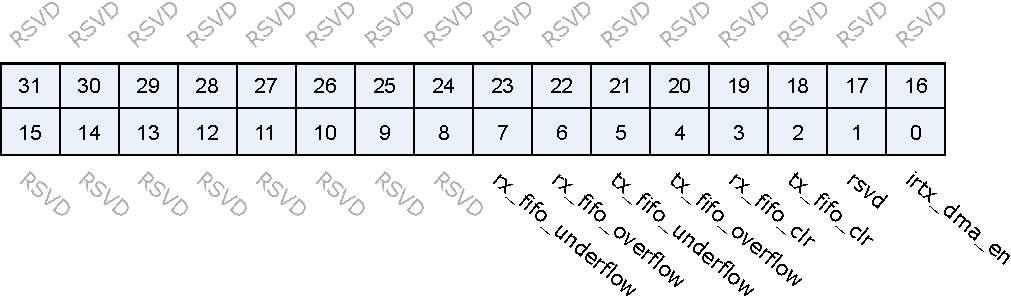
\includegraphics{ir_irtx_fifo_config_0.pdf}
\end{figure}

\regdes{31:8&RSVD& & & \\\hline
7&rx\_fifo\_underflow&r&1'b0&Underflow flag of RX FIFO, can be cleared by rx\_fifo\_clr\\\hline
6&rx\_fifo\_overflow&r&1'b0&Overflow flag of RX FIFO, can be cleared by rx\_fifo\_clr\\\hline
5&tx\_fifo\_underflow&r&1'b0&Underflow flag of TX FIFO, can be cleared by tx\_fifo\_clr\\\hline
4&tx\_fifo\_overflow&r&1'b0&Overflow flag of TX FIFO, can be cleared by tx\_fifo\_clr\\\hline
3&rx\_fifo\_clr&w1c&1'b0&Clear signal of RX FIFO\\\hline
2&tx\_fifo\_clr&w1c&1'b0&Clear signal of TX FIFO\\\hline
1&rsvd&rsvd&1'b0&\\\hline
0&irtx\_dma\_en&r/w&1'b0&Enable signal of dma\_tx\_req/ack interface\\\hline

}
\subsection{irtx\_fifo\_config\_1}
\label{ir-irtx-fifo-config-1}
Address:0x2000a684
 \begin{figure}[H]
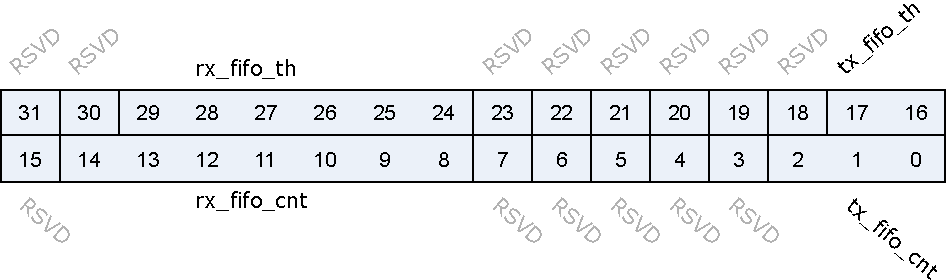
\includegraphics{ir_irtx_fifo_config_1.pdf}
\end{figure}

\regdes{31:30&RSVD& & & \\\hline
29:24&rx\_fifo\_th&r/w&6'd0&RX FIFO threshold, irrx\_frdy\_int will not be asserted if rx\_fifo\_cnt is less than this value\\\hline
23:18&RSVD& & & \\\hline
17:16&tx\_fifo\_th&r/w&2'd0&TX FIFO threshold, irtx\_frdy\_int \& dma\_tx\_req will not be asserted if tx\_fifo\_cnt is less than this value\\\hline
15&RSVD& & & \\\hline
14:8&rx\_fifo\_cnt&r&7'd0&RX FIFO available count\\\hline
7:3&RSVD& & & \\\hline
2:0&tx\_fifo\_cnt&r&3'd4&TX FIFO available count\\\hline

}
\subsection{ir\_fifo\_wdata}
\label{ir-ir-fifo-wdata}
Address:0x2000a688
 \begin{figure}[H]
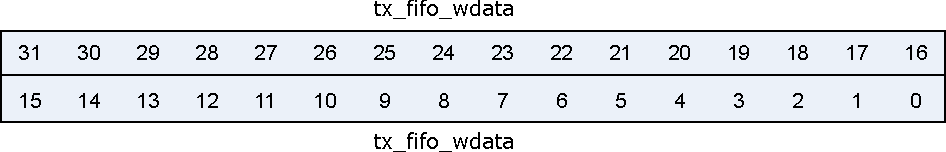
\includegraphics{ir_ir_fifo_wdata.pdf}
\end{figure}

\regdes{31:0&tx\_fifo\_wdata&w&32'h0&IRTX  FIFO data \par Normal Mode: Each entry contains a 32-bit data word, LSB is sent first \par Software Mode: Each entry contains 4 pulse widths, [7:0] is the 1st pulse, [15:8] is the 2nd pulse, etc)
\\\hline

}
\subsection{ir\_fifo\_rdata}
\label{ir-ir-fifo-rdata}
Address:0x2000a68c
 \begin{figure}[H]
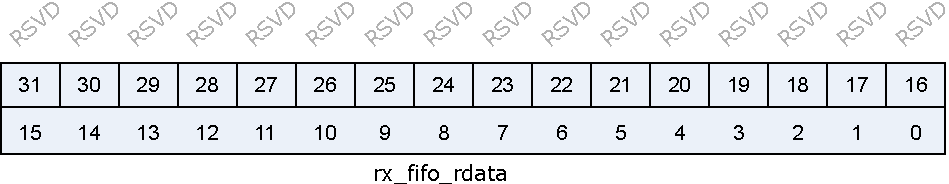
\includegraphics{ir_ir_fifo_rdata.pdf}
\end{figure}

\regdes{31:16&RSVD& & & \\\hline
15:0&rx\_fifo\_rdata&r&16'h0&IRRX FIFO pulse width data for Software Mode\\\hline

}
